% ----- Consignes exo 1 ----- %
\begin{td-exo}[Soirée chez Ramsey]\,\\ % 1 
	On considère un ensemble de six personnes. Montrer que au moins 
	trois personnes se connaissent deux-à-deux ou que au moins trois 
	personnes ne se connaissent pas deux-à-deux. 
	Est-ce vrai pour un ensemble de cinq personnes?
\end{td-exo}

% ----- Solutions exo 1 ----- %
\iftoggle{showsolutions}{
	\begin{td-sol}[]\,\\ %
		Soit \(G = (V, E)\) un graphe à six sommets. On 
		veut montrer que \(G\) contient \(K_3\) ou \(\ol{K_3}\).

		Considérons \(x\in V\) un sommet de \(G\) et procédons
		par disjonction de cas en fonction du degré de \(x\):
		\begin{itemize}
			\item Si \(\deg(x) \geq 3\), on note \(s_1, s_2, s_3\) trois voisins de \(x\).
			Si \((s_1, s_2)\in E\) alors \(x, s_1, s_2\) forment \(K_3\).
			
			De manière similaire, si \((s_1, s_3)\in E\) ou \((s_2, s_3)\in E\) alors \(K_3\) est formé.
			Si il n'existe pas d'arête entre \(s_1, s_2, s_3\) alors \(\ol{K_3}\) est formé.
			
			Ainsi, si \(\deg(x) \geq 3\) alors \(G\) contient \(K_3\) ou \(\ol{K_3}\).

			\vspace{0.1cm}
			% Figure 1
\ffigbox[\FBwidth]{
\label{Fig:td2ex9}
}{
    \fbox{
        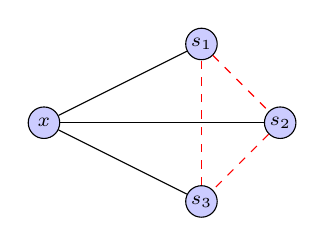
\begin{tikzpicture}[scale=1, every node/.style={circle, draw, fill=blue!20, inner sep=1pt, font=\scriptsize, minimum size=4mm}]
            \node (x) at (0, 1) {\(x\)};

            \node (s1) at (2, 2) {\(s_1\)};
            \node (s2) at (3, 1) {\(s_2\)};
            \node (s3) at (2, 0) {\(s_3\)};

            \draw (x) -- (s1);
            \draw (x) -- (s2);
            \draw (x) -- (s3);

            \draw[red, dashed] (s1) -- (s2);
            \draw[red, dashed] (s2) -- (s3);
            \draw[red, dashed] (s3) -- (s1);
        \end{tikzpicture}
    }
}

			Visuellement, on peut voir que si un des traits rouges est présent
			(donc si il existe une arête entre deux des sommets \(s_1, s_2, s_3\))
			alors \(K_3\) est formé. Sinon, il y a un triangle rouge en pointillés
			et \(\ol{K_3}\) est formé.

			\item Si \(\deg(x) \leq 2\), on note \(s_1, s_2, s_3\in V\)
			trois sommets de \(G\) qui ne sont pas voisins de \(x\) (ils
			existent forcément car \(|V| = 6\)).
			Si \((s_1, s_2)\notin E\) alors \(x, s_1, s_2\) forment \(\ol{K_3}\).

			De manière similaire, si \((s_1, s_3)\notin E\) ou \((s_2, s_3)\notin E\) alors \(\ol{K_3}\) est formé.
			Si il existe une arête entre chacun des sommets \(s_1, s_2, s_3\) alors \(K_3\) est formé.

			\vspace{0.1cm}
			\input{../assets/tikz/td_1_ex_1_case2.tex}

			Visuellement, on peut voir que si un des traits rouges est absent
			(donc si il n'existe pas d'arête entre deux des sommets \(s_1, s_2, s_3\))
			alors \(\ol{K_3}\) est formé. Sinon, il y a un triangle rouge en pointillés
			et \(K_3\) est formé.

			Ainsi, si \(\deg(x) \leq 2\) alors \(G\) contient \(K_3\) ou \(\ol{K_3}\).
		\end{itemize}
		Donc pour un ensemble de six personnes, au moins trois personnes se connaissent deux-à-deux ou au moins trois personnes ne se connaissent pas deux-à-deux.

		Pour un ensemble de cinq personnes, le graphe \(G\) à cinq sommets
		ci-dessous ne contient ni \(K_3\) ni \(\ol{K_3}\):
		\begin{center}
			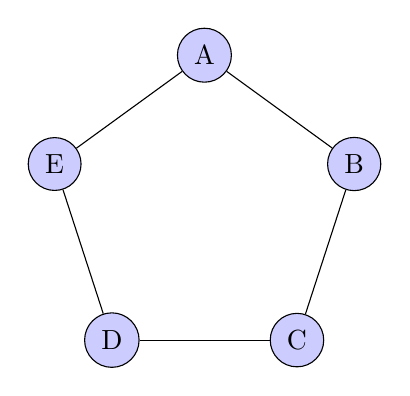
\begin{tikzpicture}[scale=1, every node/.style={circle, draw, fill=blue!20}]
				\node (A) at (90:2) {A};
				\node (B) at (18:2) {B};
				\node (C) at (-54:2) {C};
				\node (D) at (-126:2) {D};
				\node (E) at (162:2) {E};
				\foreach \from/\to in {A/B, B/C, C/D, D/E, E/A}
					\draw (\from) -- (\to);
			\end{tikzpicture}
		\end{center}
	\end{td-sol}
}{}


% ----- Consignes exo 2 ----- %
\begin{td-exo}[Hyperparcours]\,\\ % 2 
	Soit \(d\) un entier positif non nul. L'hypercube
	\(Q_d\) est le graphe dont l'ensemble des sommets est l'ensemble
	des \(d\)-uplets \(x_1,\ldots,x_d\) de 0 et de 1, deux 
	\(d\)-uplets étant adjacents s'ils diffèrent sur une seule entrée.
	\begin{enumerate}
		\item Dessiner \(Q_d\) pour \(d=1,2,3,4\).
		\item Calculer un parcours en largeur de \(Q_3\) de racine \(000\).
		En cas de choix entre plusieurs sommets pour entrer dans la file, on choisira celui
		de valeur (en binaire) minimale.
		\item Effectuer de même un parcours en profondeur de \(Q_3\).
		Cette fois, il n'y a pas de consigne en cas de choix, mais
		on essayera d'obtenir un arbre de parcours qui ne soit pas un chemin.
	\end{enumerate}
\end{td-exo}

% ----- Solutions exo 2 ----- %
\iftoggle{showsolutions}{
	\begin{td-sol}[]\, %
		\begin{enumerate}
			\item On a les hypercubes suivants:
			
			\begin{figure}[H]
	\CenterFloatBoxes{}		% centers the floatrow contents horizontally
	\begin{floatrow}
		% Figure 1
\ffigbox[\FBwidth]{
\caption{\centering \,\\Hypercube \(Q_1\)}\label{Fig:qd1}
}{
    \fbox{
        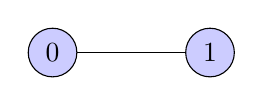
\begin{tikzpicture}[scale=1, every node/.style={circle, draw, fill=blue!20}]
            \node (A) at (0, 0) {0};
            \node (B) at (2, 0) {1};
            \foreach \from/\to in {A/B} \draw (\from) -- (\to);
        \end{tikzpicture}
    }
}

		% Figure 2
\ffigbox[\FBwidth]{
\caption{\centering \,\\Hypercube \(Q_2\)}\label{Fig:qd2}
}{
    \fbox{
        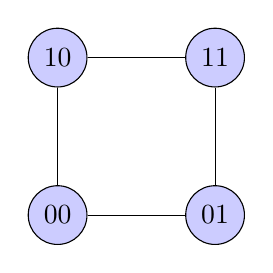
\begin{tikzpicture}[scale=1, every node/.style={circle, draw, fill=blue!20}]
            \node (A) at (0, 0) {00};
            \node (B) at (2, 0) {01};
            \node (C) at (2, 2) {11};
            \node (D) at (0, 2) {10};
            \foreach \from/\to in {A/B, B/C, C/D, D/A} \draw (\from) -- (\to);
        \end{tikzpicture}
    }
}

		% Figure 3
\ffigbox[\FBwidth]{
\caption{\centering \,\\Hypercube \(Q_3\)}\label{Fig:qd3}
}{
    \fbox{
        % Q3: Cube (Hypercube of dimension 3)
        \begin{tikzpicture}[scale=1, every node/.style={circle, draw, fill=blue!20, inner sep=1pt, font=\scriptsize}]
            % Parameters
            \def\L{2}            % side length of square
            \def\dx{0.9} \def\dy{0.6} % offset for the "back" square (gives perspective)

            % front (lower) square: coordinates ordered 000,001,011,010 (clockwise)
            \coordinate (v000) at (0,0);
            \coordinate (v001) at (\L,0);
            \coordinate (v011) at (\L,\L);
            \coordinate (v010) at (0,\L);

            % back (shifted) square: add (dx,dy) and these will be 100,101,111,110
            \coordinate (v100) at ($ (v000) + (\dx,\dy) $);
            \coordinate (v101) at ($ (v001) + (\dx,\dy) $);
            \coordinate (v111) at ($ (v011) + (\dx,\dy) $);
            \coordinate (v110) at ($ (v010) + (\dx,\dy) $);

            % draw edges front square
            \foreach \a/\b in {v000/v001, v001/v011, v011/v010, v010/v000}
                \draw (\a) -- (\b);

            % draw edges back square
            \foreach \a/\b in {v100/v101, v101/v111, v111/v110, v110/v100}
                \draw (\a) -- (\b);

            % connect corresponding vertices (cube edges)
            \foreach \a/\b in {v000/v100, v001/v101, v011/v111, v010/v110}
                \draw (\a) -- (\b);

            % nodes with labels (binary strings)
            \node at (v000) {000};
            \node at (v001) {001};
            \node at (v011) {011};
            \node at (v010) {010};
            \node at (v100) {100};
            \node at (v101) {101};
            \node at (v111) {111};
            \node at (v110) {110};
        \end{tikzpicture}
    }
}
	\end{floatrow}
\end{figure}

\begin{figure}[H]
	\CenterFloatBoxes{}		% centers the floatrow contents horizontally
	\begin{floatrow}
		% Figure 4
\ffigbox[\FBwidth]{
\caption{\centering Hypercube \(Q_4\)\\Noeuds non précisés pour la clareté}\label{Fig:qd4}
}{
    \fbox{
        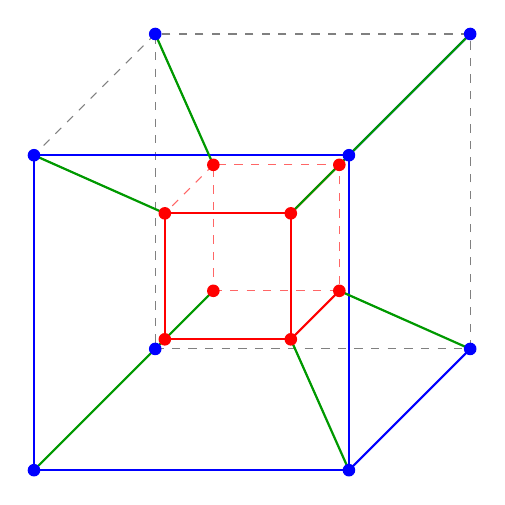
\begin{tikzpicture}[scale=2, line join=round]
            % Define the vertices of the outer cube
            \coordinate (A1) at (0,0,0);
            \coordinate (B1) at (2,0,0);
            \coordinate (C1) at (2,2,0);
            \coordinate (D1) at (0,2,0);
            \coordinate (E1) at (0,0,2);
            \coordinate (F1) at (2,0,2);
            \coordinate (G1) at (2,2,2);
            \coordinate (H1) at (0,2,2);
            
            % Define the vertices of the inner cube (offset)
            \coordinate (A2) at (0.6,0.6,0.6);
            \coordinate (B2) at (1.4,0.6,0.6);
            \coordinate (C2) at (1.4,1.4,0.6);
            \coordinate (D2) at (0.6,1.4,0.6);
            \coordinate (E2) at (0.6,0.6,1.4);
            \coordinate (F2) at (1.4,0.6,1.4);
            \coordinate (G2) at (1.4,1.4,1.4);
            \coordinate (H2) at (0.6,1.4,1.4);
            
            % Draw the outer cube (hidden edges dashed)
            \draw[dashed, gray] (A1) -- (B1) -- (C1) -- (D1) -- cycle; % bottom face
            \draw[dashed, gray] (A1) -- (E1);
            \draw[dashed, gray] (D1) -- (H1);
            \draw[blue, thick] (B1) -- (F1);
            \draw[blue, thick] (C1) -- (G1);
            \draw[blue, thick] (E1) -- (F1) -- (G1) -- (H1) -- cycle; % top face
            
            % Draw the inner cube (hidden edges dashed)
            \draw[dashed, red!60] (A2) -- (B2) -- (C2) -- (D2) -- cycle; % bottom face
            \draw[dashed, red!60] (A2) -- (E2);
            \draw[dashed, red!60] (D2) -- (H2);
            \draw[red, thick] (B2) -- (F2);
            \draw[red, thick] (C2) -- (G2);
            \draw[red, thick] (E2) -- (F2) -- (G2) -- (H2) -- cycle; % top face
            
            % Draw connecting edges between outer and inner cubes (tesseract edges)
            \draw[green!60!black, thick] (A1) -- (A2);
            \draw[green!60!black, thick] (B1) -- (B2);
            \draw[green!60!black, thick] (C1) -- (C2);
            \draw[green!60!black, thick] (D1) -- (D2);
            \draw[green!60!black, thick] (E1) -- (E2);
            \draw[green!60!black, thick] (F1) -- (F2);
            \draw[green!60!black, thick] (G1) -- (G2);
            \draw[green!60!black, thick] (H1) -- (H2);
            
            % Add small dots at vertices for clarity
            \foreach \point in {A1,B1,C1,D1,E1,F1,G1,H1}
                \fill[blue] (\point) circle (0.04);
            \foreach \point in {A2,B2,C2,D2,E2,F2,G2,H2}
                \fill[red] (\point) circle (0.04);
        \end{tikzpicture}
    }
}
	\end{floatrow}
\end{figure}

			\item On peut effectuer le parcours en largeur suivant:
			\begin{equation*}
				\begin{aligned}
					&000 \rightarrow 001 \rightarrow 010 \rightarrow 100\\
					&001 \rightarrow 011 \rightarrow 101\\
					&010 \rightarrow 110\\
					&011 \rightarrow 111
				\end{aligned}
			\end{equation*}
			ce qui se représente visuellement comme suit:

			% Figure 3
\ffigbox[\FBwidth]{
\caption{\centering \,\\Hypercube \(Q_3\)}\label{Fig:qd3}
}{
    \fbox{
        % Q3: Cube (Hypercube of dimension 3)
        \begin{tikzpicture}[scale=1, every node/.style={circle, draw, fill=blue!20, inner sep=1pt, font=\scriptsize}]
            % Parameters
            \def\L{2}            % side length of square
            \def\dx{0.9} 
            \def\dy{0.6}         % offset for the "back" square (gives perspective)
            \def\offset{0.12}    % offset distance from cube edges
            
            % front (lower) square: coordinates ordered 000,001,011,010 (clockwise)
            \coordinate (v000) at (0,0);
            \coordinate (v001) at (\L,0);
            \coordinate (v011) at (\L,\L);
            \coordinate (v010) at (0,\L);
            
            % back (shifted) square: add (dx,dy) and these will be 100,101,111,110
            \coordinate (v100) at ($ (v000) + (\dx,\dy) $);
            \coordinate (v101) at ($ (v001) + (\dx,\dy) $);
            \coordinate (v111) at ($ (v011) + (\dx,\dy) $);
            \coordinate (v110) at ($ (v010) + (\dx,\dy) $);
            
            % draw edges front square
            \foreach \a/\b in {v000/v001, v001/v011, v011/v010, v010/v000}
                \draw (\a) -- (\b);
            
            % draw edges back square
            \foreach \a/\b in {v100/v101, v101/v111, v111/v110, v110/v100}
                \draw (\a) -- (\b);
            
            % connect corresponding vertices (cube edges)
            \foreach \a/\b in {v000/v100, v001/v101, v011/v111, v010/v110}
                \draw (\a) -- (\b);
            
            % Path: 000 → 001 → 101 → 100 → 110 → 010 → 011 → 111
            % Draw arrows parallel to edges but offset outside
            
            % Arrow 1: 000 → 001 (bottom edge, offset downward)
            \draw[->, thick, red!70!black] 
                ($ (v000) + (0,-\offset) $) -- ($ (v001) + (0,-\offset) $);
            \node[draw=none, fill=none, font=\tiny, text=red!70!black] at ($ (v000)!0.5!(v001) + (0,-\offset-0.15) $) {1};
            
            % Arrow 2: 001 → 101 (right-back edge, offset to the right)
            \draw[->, thick, red!70!black] 
                ($ (v001) + (\offset,-\offset) $) -- ($ (v101) + (\offset,-\offset) $);
            \node[draw=none, fill=none, font=\tiny, text=red!70!black] at ($ (v001)!0.5!(v101) + (\offset+0.15,-\offset) $) {2};
            
            % Arrow 3: 101 → 100 (top-back edge, offset behind/up)
            \draw[->, thick, red!70!black] 
                ($ (v101) + (\offset,\offset) $) -- ($ (v100) + (\offset,\offset) $);
            \node[draw=none, fill=none, font=\tiny, text=red!70!black] at ($ (v101)!0.5!(v100) + (\offset,\offset+0.15) $) {3};
            
            % Arrow 4: 100 → 110 (left-back edge, offset behind/left)
            \draw[->, thick, red!70!black] 
                ($ (v100) + (-\offset,\offset) $) -- ($ (v110) + (-\offset,\offset) $);
            \node[draw=none, fill=none, font=\tiny, text=red!70!black] at ($ (v100)!0.5!(v110) + (-\offset-0.15,\offset) $) {4};
            
            % Arrow 5: 110 → 010 (left front-back edge, offset to the left)
            \draw[->, thick, red!70!black] 
                ($ (v110) + (-\offset,0) $) -- ($ (v010) + (-\offset,0) $);
            \node[draw=none, fill=none, font=\tiny, text=red!70!black] at ($ (v110)!0.5!(v010) + (-\offset-0.15,0) $) {5};
            
            % Arrow 6: 010 → 011 (left-top edge, offset to the right)
            \draw[->, thick, red!70!black] 
                ($ (v010) + (\offset,0) $) -- ($ (v011) + (\offset,0) $);
            \node[draw=none, fill=none, font=\tiny, text=red!70!black] at ($ (v010)!0.5!(v011) + (\offset+0.15,0) $) {6};
            
            % Arrow 7: 011 → 111 (right front-back edge, offset to the right)
            \draw[->, thick, red!70!black] 
                ($ (v011) + (\offset,0) $) -- ($ (v111) + (\offset,0) $);
            \node[draw=none, fill=none, font=\tiny, text=red!70!black] at ($ (v011)!0.5!(v111) + (\offset+0.15,0) $) {7};
            
            % nodes with labels (binary strings) - drawn last to be on top
            \node at (v000) {000};
            \node at (v001) {001};
            \node at (v011) {011};
            \node at (v010) {010};
            \node at (v100) {100};
            \node at (v101) {101};
            \node at (v111) {111};
            \node at (v110) {110};
        \end{tikzpicture}
    }
}

			\item On peut effectuer le parcours en profondeur suivant:
			\begin{equation*}
				\begin{aligned}
					&000 \rightarrow 001 \rightarrow 101 \rightarrow 111 \rightarrow 110 \rightarrow 100\\
					&100 \rightarrow 110\\
					&110 \rightarrow 010 \rightarrow 011
				\end{aligned}
			\end{equation*}
			ce qui se représente visuellement comme suit:

			\begin{figure}[H]
	\CenterFloatBoxes{}
	\begin{floatrow}
		% Figure DFS 1
\ffigbox[\FBwidth]{
\caption{\centering \,\\DFS sur \(Q_3\) --- Phase 1}\label{Fig:dfs1}
}{
    \fbox{
        \begin{tikzpicture}[scale=1, every node/.style={circle, draw, fill=blue!20, inner sep=1pt, font=\scriptsize}]
            \def\L{2}
            \def\dx{0.9} 
            \def\dy{0.6}
            \def\offset{0.15}
            
            \coordinate (v000) at (0,0);
            \coordinate (v001) at (\L,0);
            \coordinate (v011) at (\L,\L);
            \coordinate (v010) at (0,\L);
            \coordinate (v100) at ($ (v000) + (\dx,\dy) $);
            \coordinate (v101) at ($ (v001) + (\dx,\dy) $);
            \coordinate (v111) at ($ (v011) + (\dx,\dy) $);
            \coordinate (v110) at ($ (v010) + (\dx,\dy) $);
            
            % Edges
            \foreach \a/\b in {v000/v001, v001/v011, v011/v010, v010/v000}
                \draw[gray!50] (\a) -- (\b);
            \foreach \a/\b in {v100/v101, v101/v111, v111/v110, v110/v100}
                \draw[gray!50] (\a) -- (\b);
            \foreach \a/\b in {v000/v100, v001/v101, v011/v111, v010/v110}
                \draw[gray!50] (\a) -- (\b);
            
            % Path: 000 → 001 → 101 → 111 → 110 → 100
            
            % 000 → 001
            \draw[->, very thick, red!70!black] 
                ($ (v000) + (0.1,-\offset) $) -- ($ (v001) + (-0.1,-\offset) $);
            \node[draw=none, fill=white, inner sep=1pt, font=\tiny, text=red!70!black] 
                at ($ (v000)!0.5!(v001) + (0,-\offset-0.25) $) {1};
            
            % 001 → 101
            \draw[->, very thick, red!70!black] 
                ($ (v001) + (\offset,0) $) -- ($ (v101) + (\offset,0) $);
            \node[draw=none, fill=white, inner sep=1pt, font=\tiny, text=red!70!black] 
                at ($ (v001)!0.3!(v101) + (\offset+0.3,0) $) {2};
            
            % 101 → 111
            \draw[->, very thick, red!70!black] 
                ($ (v101) + (\offset,0.1) $) -- ($ (v111) + (\offset,-0.1) $);
            \node[draw=none, fill=white, inner sep=1pt, font=\tiny, text=red!70!black] 
                at ($ (v101)!0.5!(v111) + (\offset+0.25,0) $) {3};
            
            % 111 → 110
            \draw[->, very thick, red!70!black] 
                ($ (v111) + (-0.1,\offset) $) -- ($ (v110) + (0.1,\offset) $);
            \node[draw=none, fill=white, inner sep=1pt, font=\tiny, text=red!70!black] 
                at ($ (v111)!0.5!(v110) + (0,\offset+0.25) $) {4};
            
            % 110 → 100
            \draw[->, very thick, red!70!black] 
                ($ (v110) + (-\offset,0.1) $) -- ($ (v100) + (-\offset,-0.1) $);
            \node[draw=none, fill=white, inner sep=1pt, font=\tiny, text=red!70!black] 
                at ($ (v110)!0.5!(v100) + (-\offset-0.25,0) $) {5};
            
            % Nodes
            \node[fill=green!30] at (v000) {000};
            \node[fill=green!30] at (v001) {001};
            \node at (v011) {011};
            \node at (v010) {010};
            \node[fill=green!30] at (v100) {100};
            \node[fill=green!30] at (v101) {101};
            \node[fill=green!30] at (v111) {111};
            \node[fill=green!30] at (v110) {110};
        \end{tikzpicture}
    }
}

		% Figure DFS 2
\ffigbox[\FBwidth]{
\caption{\centering \,\\DFS sur \(Q_3\) --- Phase 2}\label{Fig:dfs2}
}{
    \fbox{
        \begin{tikzpicture}[scale=1, every node/.style={circle, draw, fill=blue!20, inner sep=1pt, font=\scriptsize}]
            \def\L{2}
            \def\dx{0.9} 
            \def\dy{0.6}
            \def\offset{0.15}
            
            \coordinate (v000) at (0,0);
            \coordinate (v001) at (\L,0);
            \coordinate (v011) at (\L,\L);
            \coordinate (v010) at (0,\L);
            \coordinate (v100) at ($ (v000) + (\dx,\dy) $);
            \coordinate (v101) at ($ (v001) + (\dx,\dy) $);
            \coordinate (v111) at ($ (v011) + (\dx,\dy) $);
            \coordinate (v110) at ($ (v010) + (\dx,\dy) $);
            
            % Edges
            \foreach \a/\b in {v000/v001, v001/v011, v011/v010, v010/v000}
                \draw[gray!50] (\a) -- (\b);
            \foreach \a/\b in {v100/v101, v101/v111, v111/v110, v110/v100}
                \draw[gray!50] (\a) -- (\b);
            \foreach \a/\b in {v000/v100, v001/v101, v011/v111, v010/v110}
                \draw[gray!50] (\a) -- (\b);
            
            % Previous path (lighter)
            \draw[->, thick, red!40!black] 
                ($ (v000) + (0.1,-\offset) $) -- ($ (v001) + (-0.1,-\offset) $);
            \draw[->, thick, red!40!black] 
                ($ (v001) + (\offset,0) $) -- ($ (v101) + (\offset,0) $);
            \draw[->, thick, red!40!black] 
                ($ (v101) + (\offset,0.1) $) -- ($ (v111) + (\offset,-0.1) $);
            \draw[->, thick, red!40!black] 
                ($ (v111) + (-0.1,\offset) $) -- ($ (v110) + (0.1,\offset) $);
            \draw[->, thick, red!40!black] 
                ($ (v110) + (-\offset,0.1) $) -- ($ (v100) + (-\offset,-0.1) $);
            
            % Backtracking 100 → 110 (dashed blue)
            \draw[->, very thick, blue!60!black, dashed] 
                ($ (v100) + (-\offset-0.25,-0.1) $) -- ($ (v110) + (-\offset-0.25,0.1) $);
            
            % 110 → 010 (exploration)
            \draw[->, very thick, red!70!black] 
                ($ (v110) + (-\offset,0) $) -- ($ (v010) + (-\offset,0) $);
            \node[draw=none, fill=white, inner sep=1pt, font=\tiny, text=red!70!black] 
                at ($ (v110)!0.4!(v010) + (-\offset-0.25,0.1) $) {6};
            
            % 010 → 011 (exploration)
            \draw[->, very thick, red!70!black] 
                ($ (v010) + (0.1,\offset) $) -- ($ (v011) + (-0.1,\offset) $);
            \node[draw=none, fill=white, inner sep=1pt, font=\tiny, text=red!70!black] 
                at ($ (v010)!0.8!(v011) + (0,\offset+0.25) $) {7};
            
            % Nodes
            \node[fill=green!30] at (v000) {000};
            \node[fill=green!30] at (v001) {001};
            \node[fill=green!30] at (v011) {011};
            \node[fill=green!30] at (v010) {010};
            \node[fill=green!30] at (v100) {100};
            \node[fill=green!30] at (v101) {101};
            \node[fill=green!30] at (v111) {111};
            \node[fill=green!30] at (v110) {110};
        \end{tikzpicture}
    }
}
	\end{floatrow}
\end{figure}
		\end{enumerate}
	\end{td-sol}
}{}


% ----- Consignes exo 3 ----- %
\begin{td-exo}[Biparti]\,\\ % 3 
	Montrer qu'un graphe est biparti si et seulement si il ne contient
	pas de cycle impair comme sous-graphe (on pourra s'aider 
	d'un parcours en largeur).
\end{td-exo}

% ----- Solutions exo 3 ----- %
\iftoggle{showsolutions}{
	\begin{td-sol}[]\,\\ %
		Montrons qu'un graphe est biparti si et seulement si il ne contient pas de cycle impair comme sous-graphe.
		\begin{itemize}
			\item Sens direct: Supposons que \(G\) est biparti. Soit \(C\) un cycle de \(G\).
			Par définition d'un graphe biparti, on peut colorier les sommets de \(G\)
			en deux couleurs telles que deux sommets adjacents
			n'aient pas la même couleur. En parcourant le cycle \(C\), on remarque
			que chaque sommet doit avoir une couleur différente du sommet précédent.
			Ainsi, si le cycle \(C\) a une longueur impaire, le premier et le dernier
			sommet du cycle \(C\) seraient de la même couleur, ce qui est impossible
			car ils sont adjacents. Donc \(C\) ne peut pas être de longueur impaire.

			\begin{figure}[H]
	\CenterFloatBoxes{}		% centers the floatrow contents horizontally
	\begin{floatrow}
		% Figure 1
\ffigbox[\FBwidth]{
\caption{\centering Cas cycle pair}\label{Fig:td1ex3c2}
}{
    \fbox{
        \resizebox{!}{3cm}{%
            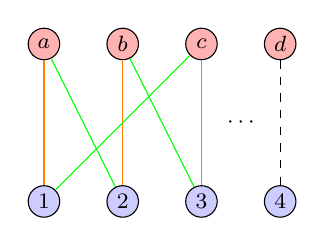
\begin{tikzpicture}[scale=1, every node/.style={circle, draw, fill=blue!20, inner sep=1pt, font=\footnotesize, minimum size=4mm}]
                \node[fill=red!30] (a) at (0, 2) {\(a\)};
                \node[fill=red!30] (b) at (1, 2) {\(b\)};
                \node[fill=red!30] (c) at (2, 2) {\(c\)};
                \node[fill=red!30] (d) at (3, 2) {\(d\)};

                \node (1) at (0, 0) {\(1\)};
                \node (2) at (1, 0) {\(2\)};
                \node (3) at (2, 0) {\(3\)};
                \node (4) at (3, 0) {\(4\)};

                \node[draw=none, fill=none] (dots) at (2.5, 1) {\(\cdots\)};

                \draw[orange] (a) -- (1);
                \draw[orange] (b) -- (2);
                \draw[orange] (c) -- (3);

                \draw[green] (1) -- (c);
                \draw[green] (2) -- (a);
                \draw[green] (3) -- (b);
                
                \draw[dashed] (d) -- (4);
            \end{tikzpicture}
        }
    }
}

		% Figure 1
\ffigbox[\FBwidth]{
\caption{\centering Cas cycle impair}\label{Fig:td1ex3c1}
}{
    \fbox{
        \resizebox{!}{3cm}{%
            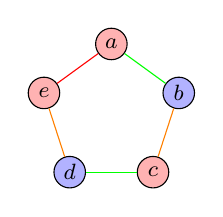
\begin{tikzpicture}[scale=0.45, every node/.style={circle, draw, fill=blue!20, inner sep=1pt, font=\footnotesize, minimum size=4mm}]
                \node[fill=red!30] (A) at (90:2) {\(a\)};
                \node[fill=blue!30] (B) at (18:2) {\(b\)};
                \node[fill=red!30] (C) at (-54:2) {\(c\)};
                \node[fill=blue!30] (D) at (-126:2) {\(d\)};
                \node[fill=red!30] (E) at (162:2) {\(e\)};

                \draw[green] (A) -- (B);
                \draw[orange] (B) -- (C);
                \draw[green] (C) -- (D);
                \draw[orange] (D) -- (E);
                \draw[red] (E) -- (A);
            \end{tikzpicture}
        }
    }
}
	\end{floatrow}
\end{figure}

			\item Sens indirect: Supposons que \(G\) ne contient pas de cycle impair.
			On choisit un sommet racine \(r\) et on effectue un BFS à partir de \(r\).
			On colorie le sommet \(r\) en rouge. Ensuite, on colorie tous les sommets
			de niveau 1 (voisins de \(r\)) en bleu, tous les sommets de niveau 2 en rouge,
			tous les sommets de niveau 3 en bleu, et ainsi de suite.

			\begin{figure}[H]
	\CenterFloatBoxes{}		% centers the floatrow contents horizontally
	\begin{floatrow}
		% Figure 1
\ffigbox[\FBwidth]{
\caption{\centering Premiere etape du BFS}\label{Fig:td_1_ex_3_2_a}
}{
    \fbox{
        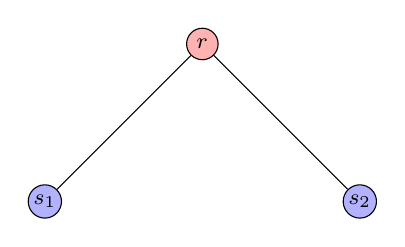
\begin{tikzpicture}[scale=1, every node/.style={circle, draw, fill=blue!20, inner sep=1pt, font=\footnotesize, minimum size=4mm}]
            \node[fill=red!30] (r) at (0, 0) {\(r\)};
            \node[fill=blue!30] (s1) at (-2, -2) {\(s_1\)};
            \node[fill=blue!30] (s2) at (2, -2) {\(s_2\)};

            \draw (r) -- (s1);
            \draw (r) -- (s2);
        \end{tikzpicture}
    }
}

		% Figure 1
\ffigbox[\FBwidth]{
\caption{\centering Deuxieme etape du BFS}\label{Fig:td1ex3c4}
}{
    \fbox{
        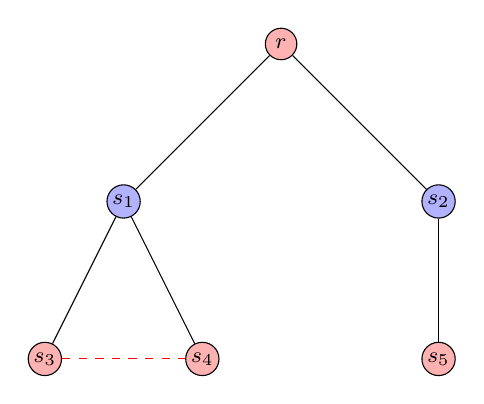
\begin{tikzpicture}[scale=1, every node/.style={circle, draw, fill=blue!20, inner sep=1pt, font=\footnotesize, minimum size=4mm}]
            \node[fill=red!30] (r) at (0, 0) {\(r\)};
            \node[fill=blue!30] (s1) at (-2, -2) {\(s_1\)};
            \node[fill=blue!30] (s2) at (2, -2) {\(s_2\)};

            \node[fill=red!30] (s3) at (-3, -4) {\(s_3\)};
            \node[fill=red!30] (s4) at (-1, -4) {\(s_4\)};
            \node[fill=red!30] (s5) at (2, -4) {\(s_5\)};

            \draw (r) -- (s1);
            \draw (r) -- (s2);

            \draw (s1) -- (s3);
            \draw (s1) -- (s4);
            \draw (s2) -- (s5);

            \draw[red, dashed] (s3) -- (s4);
        \end{tikzpicture}
    }
}
	\end{floatrow}
\end{figure}

			Si il y avait une arête entre deux sommets du même niveau, cela formerait
			un cycle impair avec le chemin passant par la racine \(r\). En effet,
			si deux sommets \(u\) et \(v\) sont au même niveau et sont adjacents,
			alors le chemin de \(r\) à \(u\), l'arête \((u,v)\), et le chemin de
			\(v\) à \(r\) forment un cycle dont la longueur est impaire (car il y a
			un nombre pair d'arêtes dans les chemins plus une arête entre \(u\) et \(v\)).
			
			Cependant, par hypothèse, \(G\) ne contient pas de cycle impair.
			Donc, il ne peut pas y avoir d'arêtes entre deux sommets du même niveau.
			Par conséquent, tous les sommets de niveau pair sont colorés en rouge et tous les sommets de niveau impair sont colorés en bleu.
			Ainsi, \(G\) est biparti.
		\end{itemize}
	\end{td-sol}
}{}


% ----- Consignes exo 4 ----- %
\begin{td-exo}[Long Chemin]\,\\ % 4 
	Montrer que tout graphe \(G\) contient un chemin de longueur \(\delta(G)\), ainsi qu'un cycle de longueur \(\geq \delta(G) + 1\) si \(\delta(G) \geq 2\). 
	Montrer que ces résultats sont optimaux.
\end{td-exo}

% ----- Solutions exo 4 ----- %
\iftoggle{showsolutions}{
	\begin{td-sol}[]\,\\ %
		Soit \(x_0\) un sommet de \(G\). On sait que \(\delta(x) \geq \delta(G)\). Il a donc au moins \(\delta(G)\) voisins. On choisit un de ces voisins, notons le \(x_1\). Ce nouveau sommet a aussi \(\delta(G)\) voisins dont au moins \(\delta(G)-1\) différents de ceux choisis précédemment. En répétant processus \(\delta(G)\) fois, on aura bien obtenu \(\delta(G)\) sommets différents de \(x_0\) et tels que \((x_0,x_1,\ldots,x_{\delta(G)})\) forme un chemin de longueur \(\delta(G)\).

		On reprend le chemin \((x_0,x_1,\ldots,x_{\delta(G)})\) choisi précédemment. Si \(x_{\delta(G)}\) est de degré 
	\end{td-sol}
}{}


% ----- Consignes exo 5 ----- %
\begin{td-exo}[Convexité]\,\\ % 5 
	% fill
\end{td-exo}

% ----- Solutions exo 5 ----- %
\iftoggle{showsolutions}{
	\begin{td-sol}[]\,\\ %
		A remplir %TODO solve exercise 5
	\end{td-sol}
}{}


% ----- Consignes exo 6 ----- %
\begin{td-exo}[Convexité]\,\\ % 6 
	% fill
\end{td-exo}

% ----- Solutions exo 6 ----- %
\iftoggle{showsolutions}{
	\begin{td-sol}[]\,\\ %
		A remplir %TODO solve exercise 6
	\end{td-sol}
}{}


% ----- Consignes exo 7 ----- %
\begin{td-exo}[Convexité]\,\\ % 7 
	% fill
\end{td-exo}

% ----- Solutions exo 7 ----- %
\iftoggle{showsolutions}{
	\begin{td-sol}[]\,\\ %
		A remplir %TODO solve exercise 7
	\end{td-sol}
}{}


% ----- Consignes exo 8 ----- %
\begin{td-exo}[Convexité]\,\\ % 8 
	% fill
\end{td-exo}

% ----- Solutions exo 8 ----- %
\iftoggle{showsolutions}{
	\begin{td-sol}[]\,\\ %
		A remplir %TODO solve exercise 8
	\end{td-sol}
}{}


% ----- Consignes exo 9 ----- %
\begin{td-exo}[Convexité]\,\\ % 9 
	% fill
\end{td-exo}

% ----- Solutions exo 9 ----- %
\iftoggle{showsolutions}{
	\begin{td-sol}[]\,\\ %
		A remplir %TODO solve exercise 9
	\end{td-sol}
}{}


% ----- Consignes exo 10 ----- %
\begin{td-exo}[Convexité]\,\\ % 10 
	% fill
\end{td-exo}

% ----- Solutions exo 10 ----- %
\iftoggle{showsolutions}{
	\begin{td-sol}[]\,\\ %
		A remplir %TODO solve exercise 10
	\end{td-sol}
}{}


% ----- Consignes exo 11 ----- %
\begin{td-exo}[Convexité]\,\\ % 11 
	% fill
\end{td-exo}

% ----- Solutions exo 11 ----- %
\iftoggle{showsolutions}{
	\begin{td-sol}[]\,\\ %
		A remplir %TODO solve exercise 11
	\end{td-sol}
}{}
